\chapter{Object Selection}\label{cha:object_selection}

For any physics analysis in proton-proton collisions at the LHC the particles traversing the ATLAS detector
need to be reconstructed and identified.
For this information of the inner detector, calorimeters, and the muon spectrometer is used.
The reconstruction is done both on data and simulation. Differences in reconstruction, identification, and trigger efficiencies are
measured and correction factors (\emph{scale factors}) are applied to the simulated events.

First, a brief overview of the reconstruction of tracks and vertices is given in \cref{sec:object_selection:tracks_and_vertices}, which
is fundamental to the reconstruction of all other objects.
Since this analysis is focusing on the \Httllfull{} decay, the reconstruction and identification of electrons and muons
is essential and described in \cref{sec:object_selection:electrons,sec:object_selection:muons}.
Additional jets in the events are used to define a VBF and boosted topology and to suppress background (\cref{sec:event_selection:categorization}).
Their reconstruction is explained in \cref{sec:object_selection:jets} as well as the identification of jets originating from B-hadrons.
The identification of hadronically decaying $\tau$-leptons (\cref{sec:object_selection:tau_leptons}) is used to suppress additional background.
Due to the four neutrinos in the final state the reconstruction of the missing transverse energy (\cref{sec:object_selection:missing_transverse_energy})
is also necessary.
The chapter closes with \cref{sec:object_selection:overlap_removal}, where the removal of the overlap between objects is explained.

\section{Tracks and Vertices}\label{sec:object_selection:tracks_and_vertices}

Particle trajectories (\emph{tracks}) are the fundamental ingredient for the reconstruction and identification
of other physics objects, which are discussed in the following sections.
The tracks are reconstructed in the inner detector by using various track reconstruction algorithms~\cite{ATL-SOFT-PUB-2007-007}.
Information of the several ID sub-detector systems (IBL, Pixel, SCT, TRT) are taken into account.
The transverse momentum and the sign of the charge of the track is calculated from the curvature of the track in the magnetic field.
Quality criteria which are based on the number of hits in the sub-detectors depending on the transverse momentum $\pt$ and pseudorapidity $\eta$
are applied.

Tracks can be used to reconstruct the primary and secondary interaction points (\emph{vertices}).
For this the tracks are extrapolated back to the interaction point to check for intersections between different tracks.
Since multiple interactions are expected during one bunch crossing (\emph{pile-up}) there are also multiple vertices, which
are reconstructed.
The vertex with the highest $\sum p_{\text{T},\text{track}}^2$ is chosen as the primary vertex, which corresponds to the
point where the interaction was the hardest.

Detailed information about tracking and vertexing in ATLAS for \runtwo{} of the LHC
can be found in~\cite{ATL-PHYS-PUB-2015-051,ATL-PHYS-PUB-2015-006,ATL-PHYS-PUB-2015-026}.


\section{Electrons}\label{sec:object_selection:electrons}

Electrons can be identified by matching clusters of energy depositions in the electromagnetic calorimeter with
extrapolations to the calorimeter of reconstructed tracks provided by the ID\@.
To suppress background contributions from pile-up events or other objects like jets and hadronically decaying $\tau$-leptons
additional information of the ID and hadronic calorimeter are considered.
The identification algorithm~\cite{ATLAS-CONF-2016-024}, a likelihood-based method, uses a multivariate analysis (MVA) technique to
combine and evaluate all provided information.
Different requirements on the likelihood discriminant\footnote{The discriminant is defined as
$\frac{\mathcal{L}_S}{\mathcal{L}_S + \mathcal{L}_B}$, where $\mathcal{L}_S$ and $\mathcal{L}_B$ denote the product of
the signal and background probability density functions of the used variables.} yield different operating points,
labeled as  \emph{loose}, \emph{medium}, and \emph{tight}.
They provide a different level of electron identification efficiency and background rejection.

In this analysis the \emph{loose} criterion is chosen.
Additional requirements are $\pt > \unit[15]{GeV}$ and $\abs{\eta} < 2.47$.
The Pixel Detector and SCT can only provide information for reconstruction and identification in this $\eta$-range.
Electrons within $1.37 < \abs{\eta} < 1.52$ are excluded, because of the poor reconstruction and identification
performance caused by the transition region between the barrel and end-cap calorimeters.

To increase the background rejection, isolation requirements are introduced by the following two discriminating variables.
The calorimetric isolation energy $\et^{\text{cone}0.2}$ is defined as the sum of transverse energy deposited within
$\dr = 0.2$ around the electron candidates.
Corrections for electron energy leakage, pile-up, and the underlying event activity are applied.
The sum of the transverse momentum of all tracks within $\dr = \min(0.2, \unit[10]{GeV} / \et)$ builds the
track isolation $\pt^{\text{varcone}0.2}$. The tracks need to fulfill certain quality requirements and have to originate
from the primary vertex.
Based on different selection criteria on the quantities $\et^{\text{cone}0.2} / \et$ and
$\pt^{\text{varcone}0.2} / \et$ multiple operating points are constructed. This analysis uses the \emph{gradient}
isolation criterion with a targeted efficiency of
$\unit[0.1143]{\%} \times \et / \text{GeV} + \unit[92.14]{\%}$~\cite{ATLAS-CONF-2016-024}.

The efficiencies of the electron identification and isolation criteria are measured using a \emph{tag-and-probe} technique
in $\Z \to \epem$ and $\JPsi \to \epem$ events~\cite{ATLAS-CONF-2016-024}.
%The \emph{tag} electron must pass the \emph{tight} identification criterion as well as some other selection criteria.
%Because of the chosen events it is very probable that a second electron, the \emph{probe}, is contained in this event.
%By counting how many \emph{probe} electrons pass the different identification and isolation requirements the efficiencies
%of those working points can be obtained.
The combined reconstruction and identification efficiencies in $\Z \to \epem$ events as a function of $\et$ and $\eta$
are shown in \cref{fig:object_selection:el_id_eff}.
To account and correct for differences in data and simulated events the efficiencies are calculated for both event types.
The ratio is then used to derive \emph{scale factors}, which are applied to the simulated events in this analysis.

\begin{figure}
    \centering
    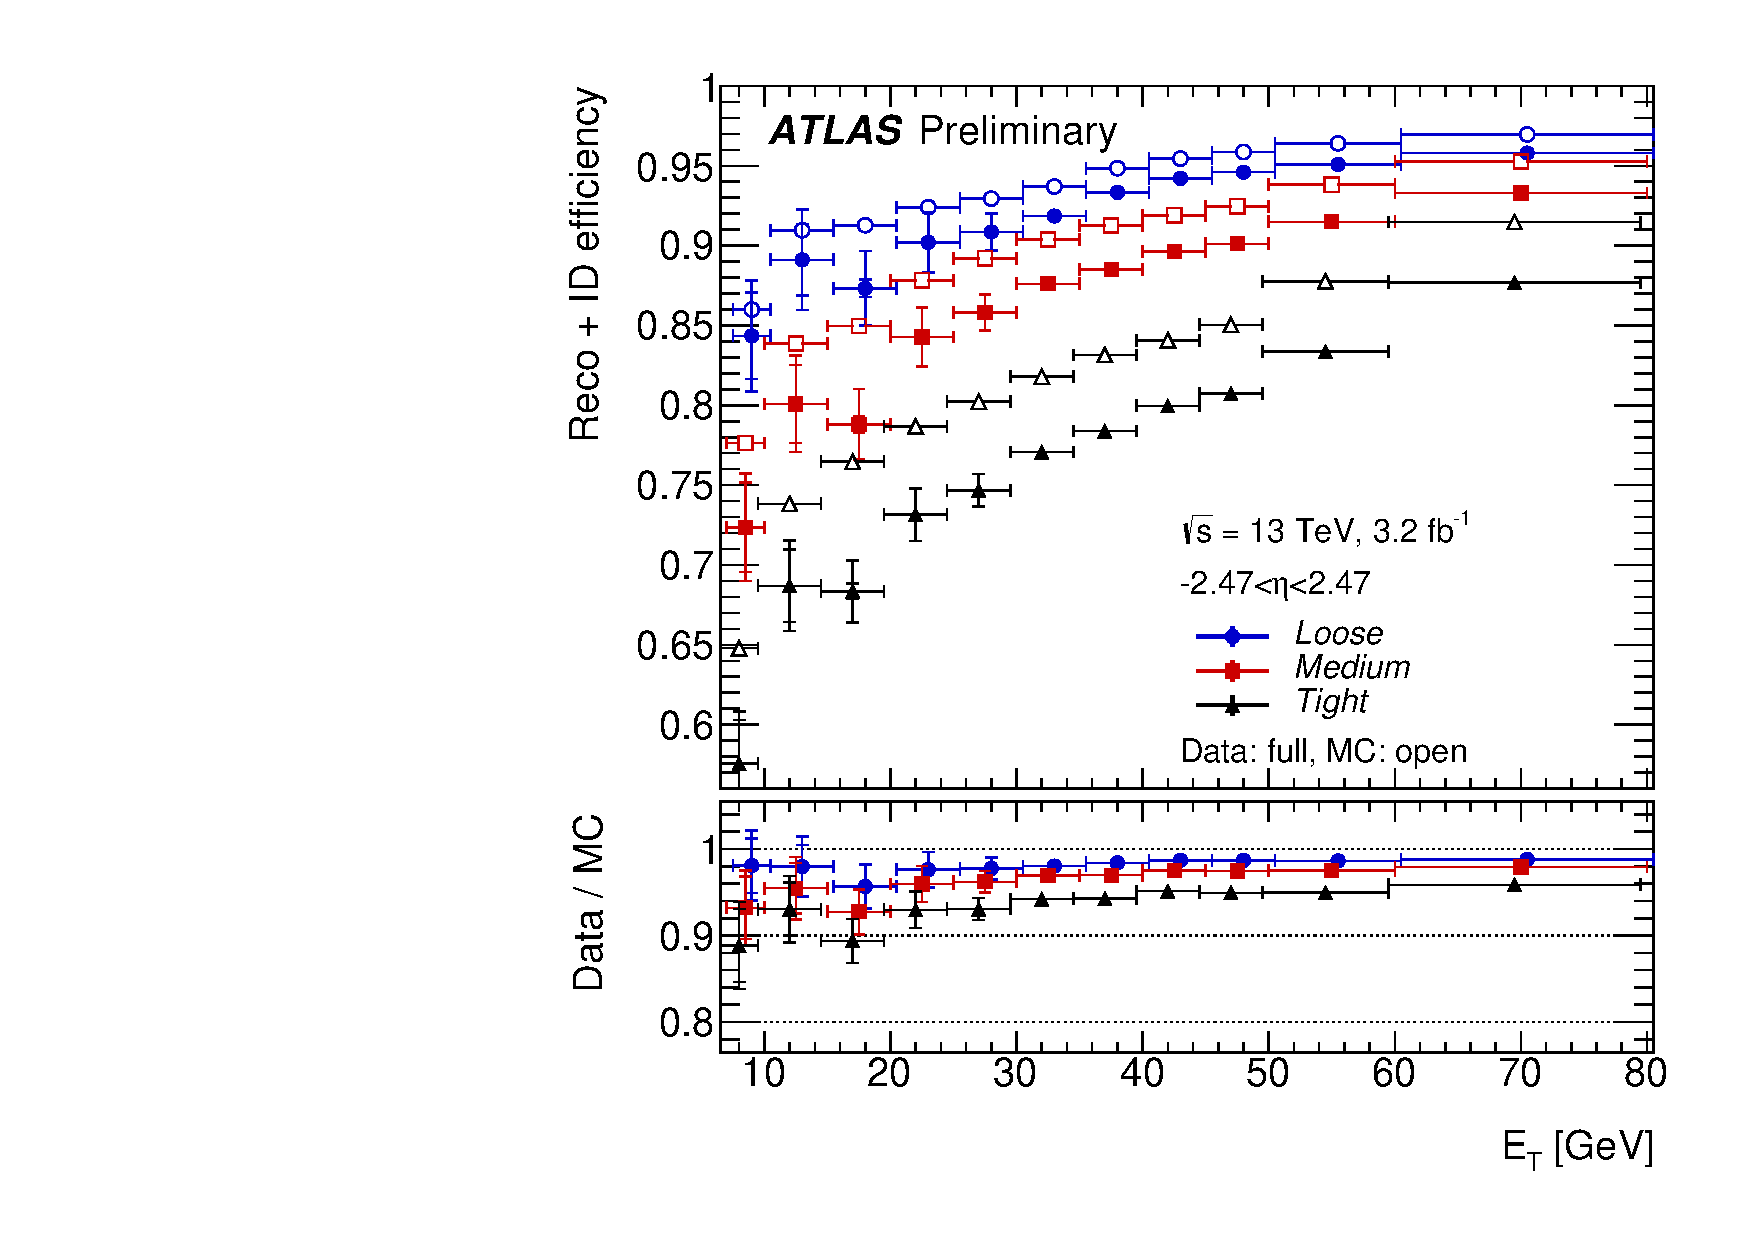
\includegraphics[width=0.45\textwidth]{./figures/object_selection/electron_efficiency_et.pdf}
    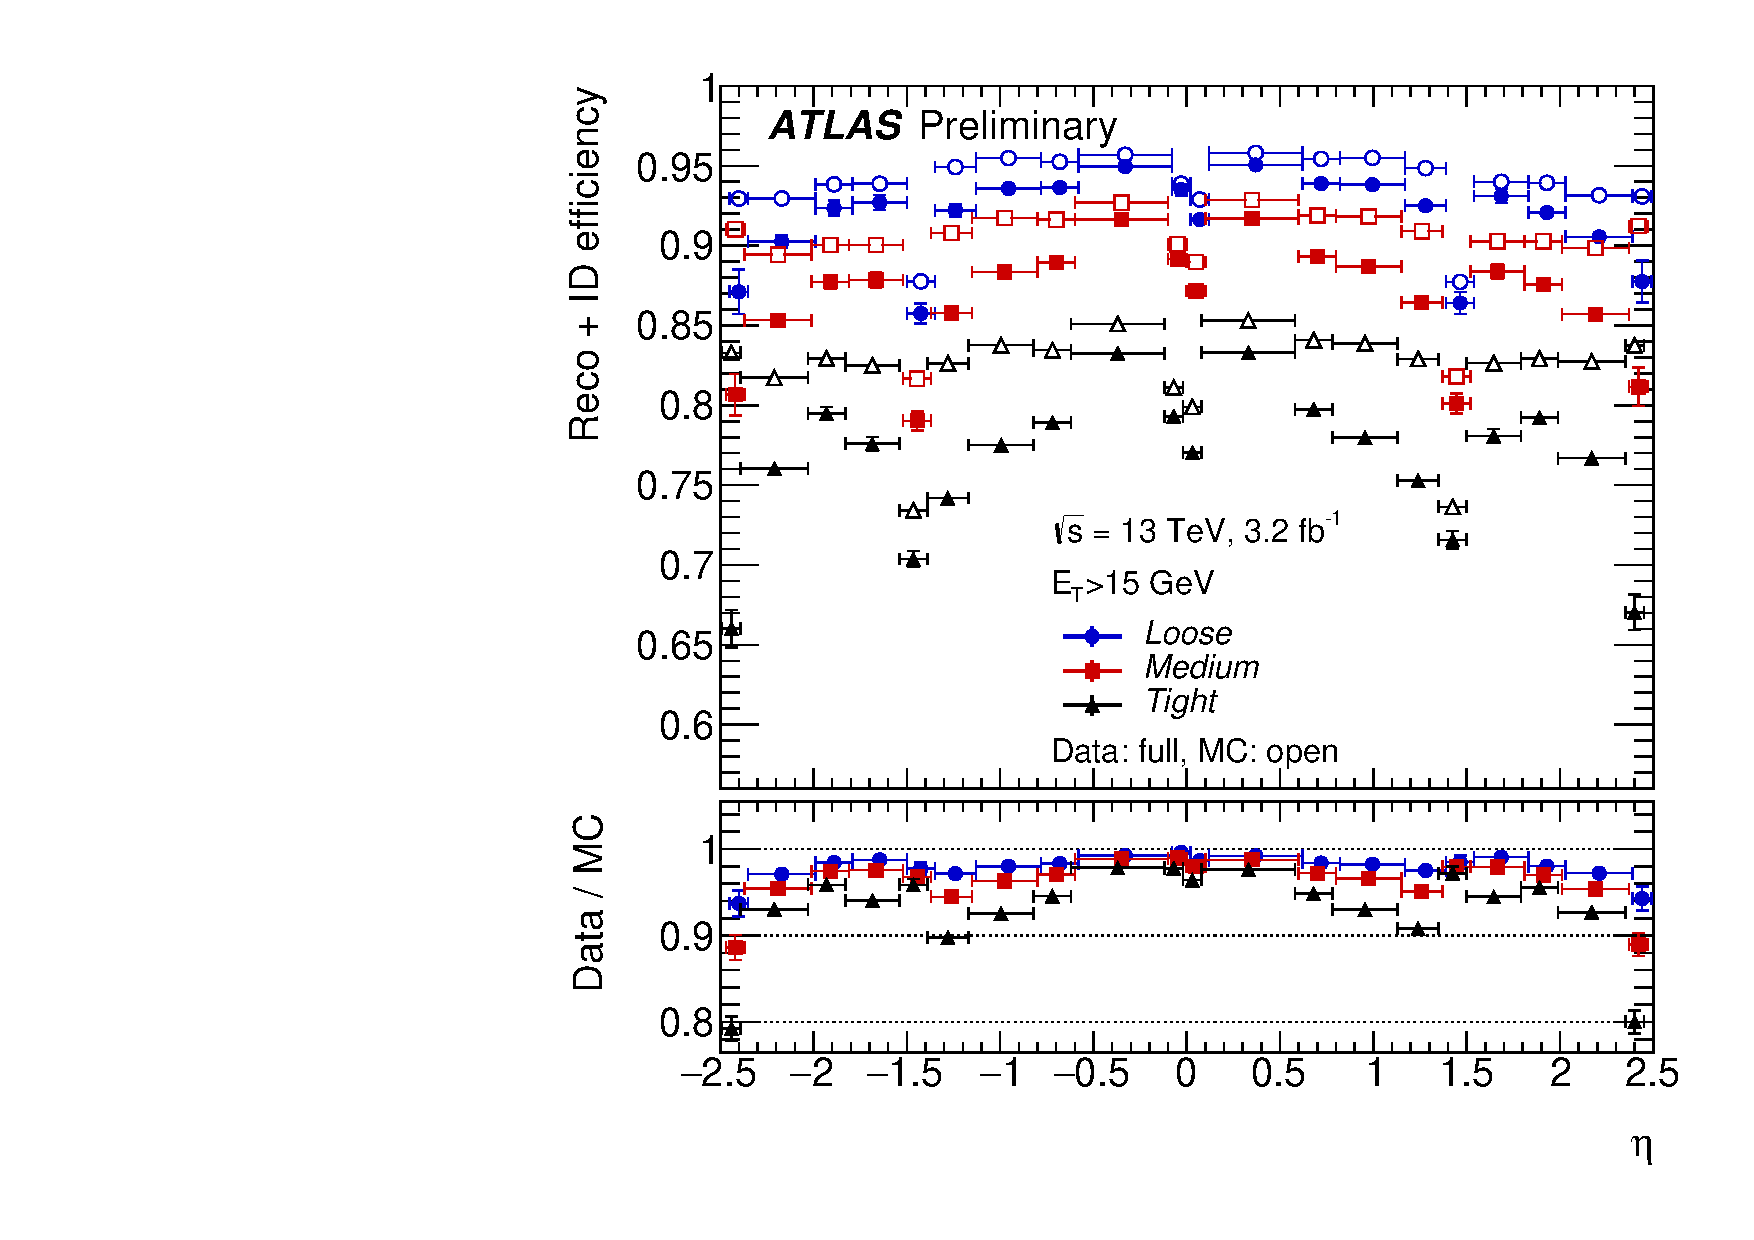
\includegraphics[width=0.45\textwidth]{./figures/object_selection/electron_efficiency_eta.pdf}
    \caption{Combined electron reconstruction and identification efficiencies for $\Z \to \epem$ events as a
             function of $\et$ (left) and $\eta$ (right) for the \emph{loose}, \emph{medium}, and \emph{tight}
             working points. The inner error bars show the statistical uncertainty, the outer error bars combine
             the statistical and systematic uncertainties.~\cite{ATLAS-CONF-2016-024}}\label{fig:object_selection:el_id_eff}
\end{figure}

\section{Muons}\label{sec:object_selection:muons}

Muons are reconstructed by taking information of the inner detector, calorimeter, and the
muon spectrometer into account.
Because  muons traverse the detectors with minimum energy loss, they have a clear signature in the detectors and the
discrimination between them and other physics objects like electrons and jets reaches a high accuracy.

First, muons are reconstructed independently in the ID and the MS\@.
For the track reconstruction in the MS each muon chamber is searched for hit patterns, which are combined to track
segments. The segments are then combined to muon track candidates. For each track candidate a global $\chi^2$ fit
is performed to the hits associated with the track. If a certain threshold is reached the track is accepted~\cite{PERF-2015-10}.

After the individual reconstruction four different algorithms are applied to combine the information of the different
sub-detector systems.
Combined (CB) muons have both a track in the ID and MS\@. The global track is calculated by a refit to both tracks.
If there is only one local track segment in the MDT or CSC chambers and the track of the ID can be extrapolated to the MS
the muon is classified as segment-tagged (ST).
A track in the ID can be classified as calorimeter-tagged (CT) muon if the track can be matched to a energy deposition
in the calorimeter, in the case that the energy deposition has the signature of a minimum-ionizing particle.
Extrapolated (ME) muons are reconstructed only from tracks in the MS with the additional requirement that the track
needs to originate from the interaction point.

To reduce background from mainly pion and kaon decays, different muon identification criteria are defined, called
\emph{loose}, \emph{medium}, and \emph{tight}.
For \emph{medium} muons only CB and ME tracks are used with some additional requirements on the number of hits in
different layers and the \emph{q/p significance}\footnote{The \emph{q/p significance} is the absolute value of the
difference between charge and momentum measured in ID and MS divided by the sum of squares of the respective uncertainties.}.
In this analysis \emph{loose} muons are used with $\pt > \unit[10]{GeV}$ and $\abs{\eta} < 2.5$.
This includes all \emph{medium} muons as well as CT and ST muons, which are however restricted to $\abs{\eta} < 0.1$.

Isolation requirements can further reduce background, because muons originating from heavy particles like $\W$, $\Z$,
or Higgs bosons are often produced isolated. Two discriminating variables are introduced.
The calorimetric isolation energy $\et^{\text{topocone}20}$ is defined as the sum of transverse energy deposited within
$\dr = 0.2$ around the muon candidates.
Corrections for pile-up and the underlying event activity are applied.
The sum of the transverse momentum of all tracks with $\pt > \unit[1]{GeV}$ within $\dr = \min(0.3, \unit[10]{GeV} / \pt^\mu)$
is defined as the track isolation $\pt^{\text{varcone}0.3}$.
Based on different selection criteria on the quantities $\et^{\text{topocone}20} / \pt^\mu$ and
$\pt^{\text{varcone}30} / \pt^\mu$ multiple operating points are constructed.
This analysis uses the \emph{gradient} isolation criterion which provides an efficiency of more than
$\unit[90(99)]{\%}$ at $\unit[20(60)]{GeV}$~\cite{PERF-2015-10}.

The muon reconstruction and identification efficiencies are obtained with a \emph{tag-and-probe} technique using
$\Z \to \mpmm$ and $\JPsi \to \mpmm$ events~\cite{PERF-2015-10}.
\cref{fig:object_selection:mu_id_eff} shows the reconstruction efficiencies for \emph{medium} and \emph{loose} muons.
The efficiencies are calculated both in data and simulated events in order to derive \emph{scale factors}, which are
applied to the simulated events to correct deviations of the efficiencies between data and simulation.

\begin{figure}
    \centering
    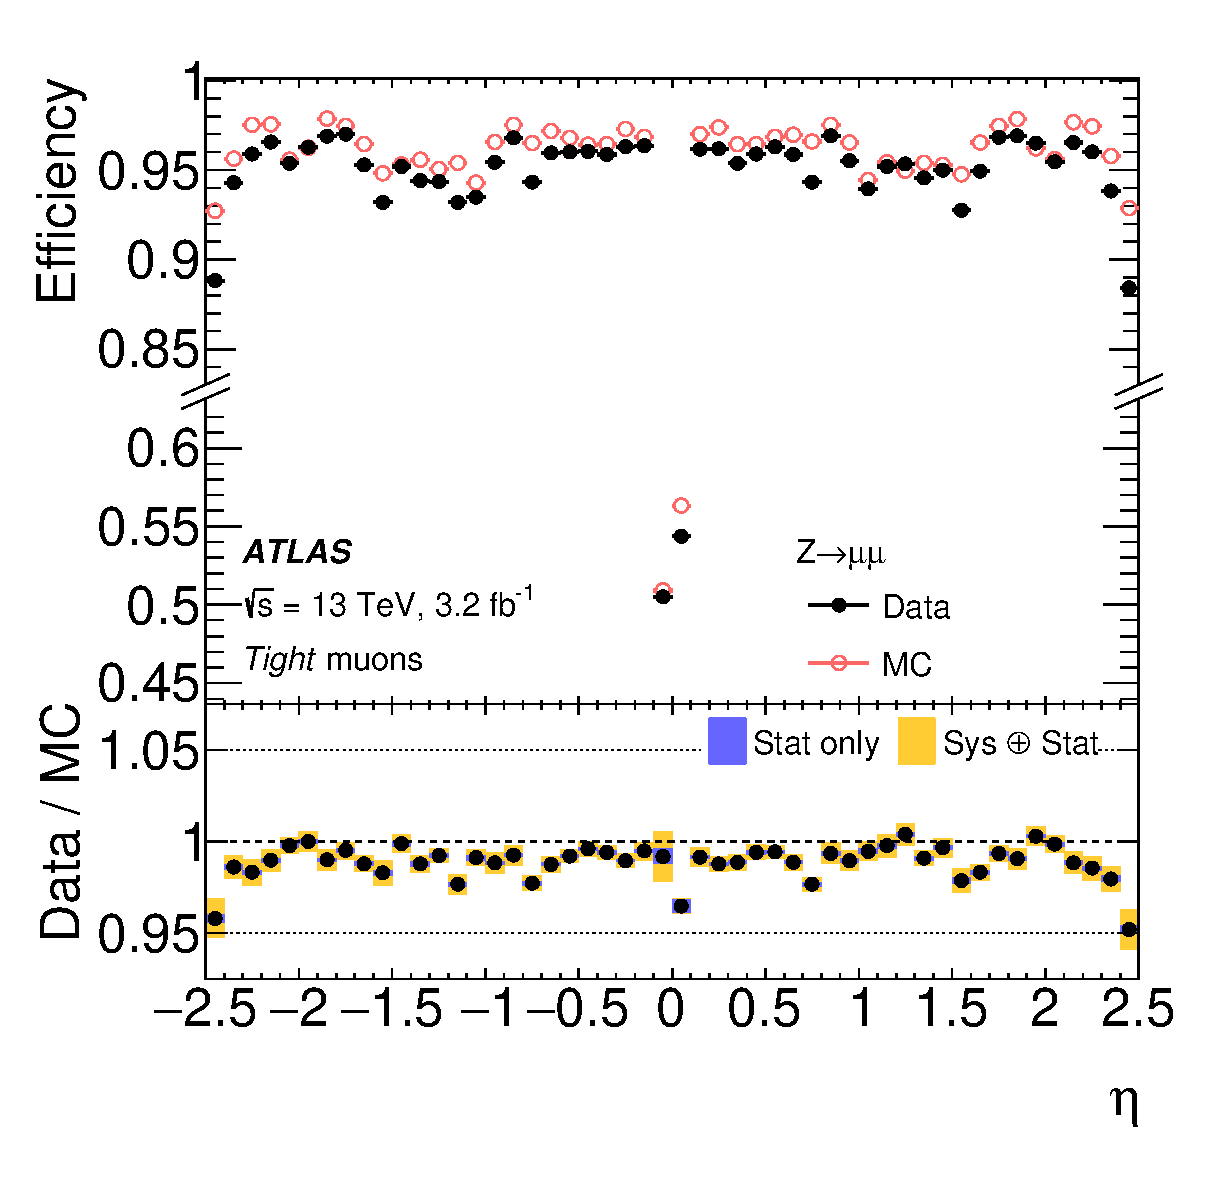
\includegraphics[width=0.45\textwidth,align=c]{./figures/object_selection/muon_efficiency_mediumloose_zmm.eps}
    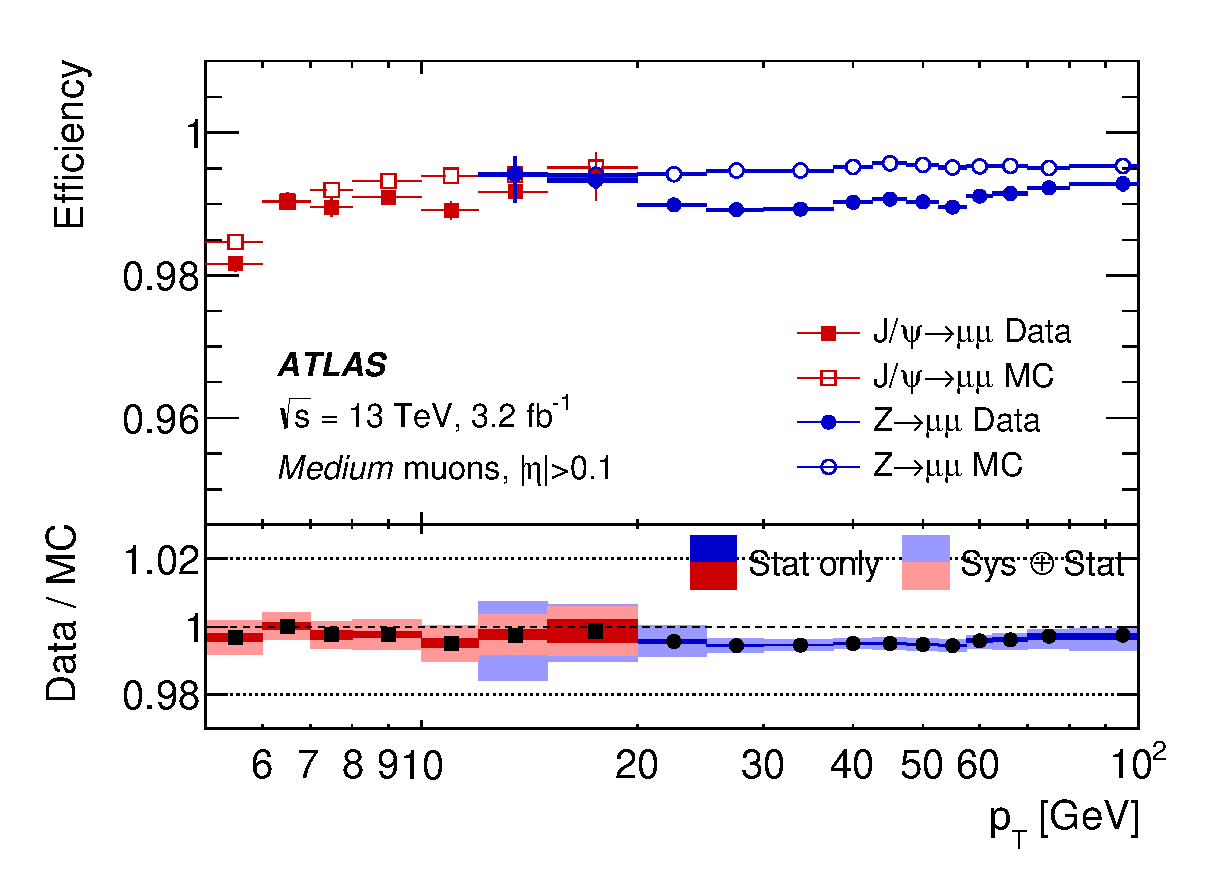
\includegraphics[width=0.45\textwidth,align=c]{./figures/object_selection/muon_efficiency_medium_zmmjpsi.eps}
    \caption{Muon reconstruction efficiencies for \emph{loose} and \emph{medium} muons as a function of $\eta$
            measured in $\Z \to \mpmm$ events (left) and for \emph{medium} muons as a function of $\pt$ measured in
            $\Z \to \mpmm$ and $\JPsi \to \mpmm$ events (right).~\cite{PERF-2015-10}}\label{fig:object_selection:mu_id_eff}
\end{figure}


\section{Jets}\label{sec:object_selection:jets}

Particles with a color charge like quarks and gluons cannot exist in an unbound state,
they form colorless states due to hadronization.\todo{Ref.\ to theory chapter}\
Collimated bunches of hadrons are produced, which are called \emph{jets}.

An algorithm which reconstructs jets should be insensitive to soft radiation (\emph{infrared safety})
and splitting of the initial seed (\emph{collinear safety}).
There are two types of jet reconstruction algorithms, cone type and sequential clustering algorithms.
Cone type algorithms use a geometrical cone around a jet axis to reconstruct the jet. In the past not
all cone algorithms were infrared and collinear safe.
Sequential cluster algorithms combine different object based on their energy and angular properties.
They provide infrared and collinear safety by construction.

In this analysis the \antikt{}~\cite{Cacciari:2008gp,Cacciari:2005hq} sequential clustering algorithm, based on energy clusters in the
hadronic calorimeter, with a distance parameter of $R = 0.4$ is used for jet reconstruction.
Not all jets are considered in the analysis, only jets with $\pt > \unit[20]{GeV}$ and $\abs{\eta} < 4.5$ are used.

The jet four-momenta undergo a series of corrections~\cite{PERF-2016-04}, to take several insufficiencies into account.
First, the jet origin is corrected to point back to the primary vertex. Next excess energy due to pile-up is removed.
Truth information of simulated dijet events is used to correct the jet energy scale (JES).
Additional JES corrections are performed in the \emph{global sequential calibration}, which uses calorimeter, muon
spectrometer and track-based variables. Finally an \emph{in-situ} correction in data is applied, using events
in $\Z+jets$, $\gamma + jets$, and dijet processes.
These corrections raise a list of systematic uncertainties, which are discussed in \cref{cha:systematic_uncertainties}.\todo{Possibly fix ref to section}

\emph{Pile-up} jets can be suppressed with the output of the jet vertex tagger (JVT) algorithm~\cite{PERF-2014-03}, which
uses tracking and vertexing information to distinguish jets from hard- and soft-scatter interactions.
All jets in this analysis with $\pt < \unit[50]{GeV}$ and $\abs{\eta} < 2.4$ are required to have $\abs{\text{JVT}} > 0.59$, where the output of the
JVT algorithm is also labeled JVT\@.
In the forward region a special algorithm for forward jets (fJVT) is used~\cite{ATL-PHYS-PUB-2015-034}.
For this analysis jets with $\pt < \unit[50]{GeV}$ and $\abs{\eta} > 2.5$ need to pass the fJVT algorithm with
$\text{fJVT} > 0.4$.
\\[\baselineskip]
Jets originating from $b$-quarks, also called $b$-jets, can be identified with \emph{$b$-tagging} algorithms.
These algorithms exploit the fact that $b$-flavoured hadrons (B-hadrons) have quite a long mean life time
($\tau \approx \unit[1.5]{ps}$~\cite{PDG}) compared to other hadrons.
The decay creates a secondary vertex several millimeters away from the primary vertex due to time
dilation.\footnote{If a lifetime of $\tau = \unit[1.5]{ps}$ and rest mass of $m_0 = \unit[5.3]{GeV}$ are assumed (approximate values, taken from~\cite{PDG}),
the B-hadron travels $c\tau' = c \tau \gamma = c \tau \frac{E}{m_0} = \unit[4.24]{mm}$ in the laboratory frame, if it has an energy of $E = \unit[50]{GeV}$.}.
The secondary vertex is reconstructed with the tracks of the charged particles which formed the jet.

Since this analysis focuses on the gluon--gluon fusion and VBF production modes of the Higgs boson, jets produced from
the decay of a $b$-quark are not expected.
However, top quarks, which produce a large background in this analysis, almost always decay into $b$-quarks
Therefore, identifying jets originating from $b$-Hadrons gives the possibility to reduce the background produced by top quarks.

This analysis uses the multivariate-based $b$-tagging algorithm MV2c20~\cite{PERF-2012-04,ATL-PHYS-PUB-2016-012} with
a working point resulting in \unit[85]{\%} efficiency for $b$-jets in simulated $t\overline{t}$ events.
The comparison to data is used to calculate tagging and mis-tagging correction factors.
The requirements of $\pt > \unit[25]{GeV}$ and $\abs{\eta} < 2.4$ are additionally applied to the $b$-tagged jets.


\section{Hadronically decaying  $\tau$-leptons}\label{sec:object_selection:tau_leptons}

Tau leptons can either decay into leptons ($\tau \to \ell \nu_\tau \nu_\ell$, $\ell = e, \mu$) or hadrons
($\tau \to \text{hadrons}$, denoted as \tauhad{}).
With a mass of \unit[1.777]{GeV} and a proper decay length of $\unit[87]{\mu m}$~\cite{PDG}, the decay usually happens before
the $\tau$-lepton reaches the active part of the ID\@.

Leptonically decaying $\tau$-leptons are identified as electrons ore muons, only hadronically decaying $\tau$-leptons can be reconstructed,
Most of the time the decay products are either one ore three charged pions, an additional neutral pion can also be produced.
Depending on the number of charged pions, the event is called either \emph{1-} or \emph{3-pronged}.
All visible decay products are denoted as \tauhadvis{}.

Since this analysis is focusing on the \Httllfull{} decay, no hadronically decaying $\tau$-leptons are expected.
However a veto on $\tauhadvis$ candidates can be used to reduce background (see \cref{sec:event_selection:preselection}).

The reconstruction starts by selecting jets which are reconstructed by using the \antikt{} algorithm~\cite{Cacciari:2008gp,Cacciari:2005hq}
with an distance parameter of $\dr = 0.4$.
Only jets with $\pt > \unit[10]{GeV}$ and $\abs{\eta} < 2.5$ are considered.
$\tauhadvis$ candidates within the transition region of the barrel end-cap calorimeters ($1.37 < \abs{\eta} < 1.52$) are discarded.
A tau vertex is calculated from the associated tracks ($\dr < 0.2$, $\pt > \unit[1]{GeV}$) of the $\tauhadvis$ candidates.
The $\eta$-$\phi$ direction is determined with information from the calorimeters. % actually: TopoCLusters
The mass and all mass related variables are set to zero.
The energy is  obtained by a tau-specific calibration scheme~\cite{Run1TauPaper}.

Quark- and gluon-initiated jets have a more broader shower profile than jets caused by $\tau$-leptons.
This can be used to distinguish between the origin of the jets.
For this a Boosted Decision Tree (BDT) based method is used.
The BDT provides multiple working points labeled as \emph{loose}, \emph{medium}, and \emph{tight}
with a targeted efficiency of $0.6$ ($0.5$), $0.55$ ($0.4$), and $0.45$ ($0.35$) for 1(3)-pronged \tauhadvis{} candidates, respectively.

In this analysis the \tauhadvis{} candidates need to pass the \emph{loose} working point, with the additional requirements
of $\pt > \unit[20]{GeV}$ and $\abs{\eta} < 2.5$.
Candidates within $1.37 < \abs{\eta} < 1.52$ are excluded.

Since the BDT was trained to discriminate between quark- and gluon-initiated jets and jets from $\tau$-leptons, it
does not perform well with regard to discriminating between 1-pronged hadronic $\tau$ decays and electrons.
A likelihood discriminator~\cite{Run1TauPaper} is build to act as an \emph{electron veto}, which uses the shower shape in the calorimeter
and track information provided by the ID, including the TRT\@.

The reconstruction and identification efficiencies as well as the trigger efficiency of hadronically decaying $\tau$-leptons is measured in
$\Z \to \tau_\mu \tauhad$ events with a \emph{tag-and-probe} technique.
The tau trigger efficiency can also be measured in $\ttbar \to \left[b\mu\nu_\mu\right]\left[b\tau\nu_\tau\right]$ events
with a similar \emph{tag-and-probe} method.
To account for differences of efficiencies in data and simulation correction factors (scale factors) are derived and applied to simulated
events.~\cite{ATL-PHYS-PUB-2015-045,ATLAS-CONF-2017-029}
The efficiencies and scale factors for 1-pronged tau decays are illustrated in \cref{fig:object_selection:tau_eff}.

\begin{figure}
    \centering
    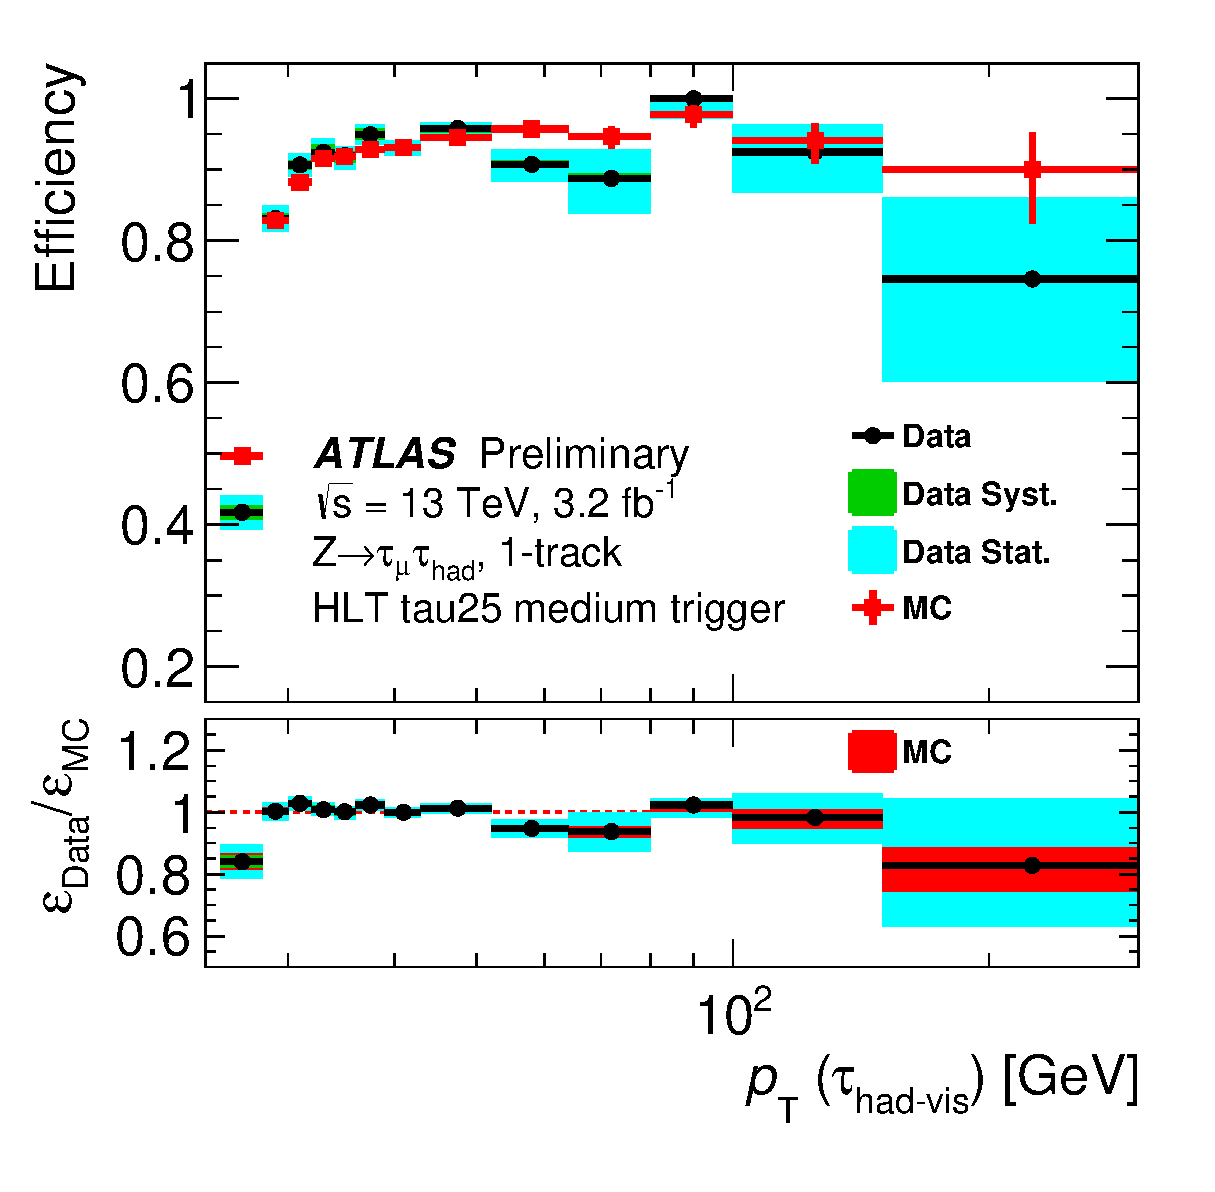
\includegraphics[width=0.45\textwidth]{./figures/object_selection/tau_trig_eff_ztt_1p.eps}
    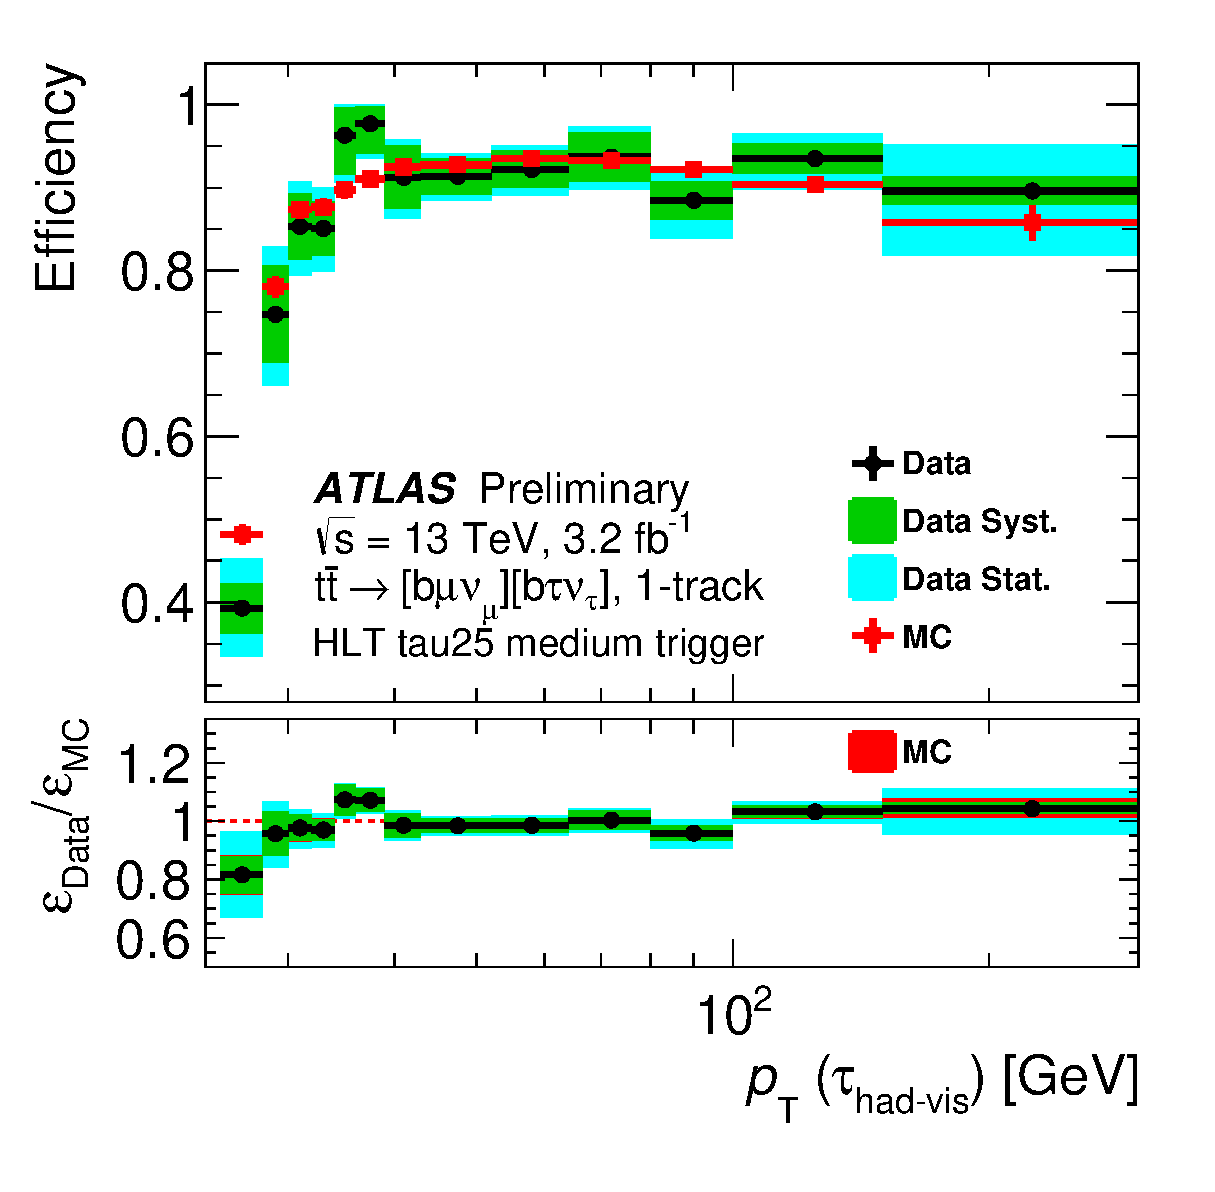
\includegraphics[width=0.45\textwidth]{./figures/object_selection/tau_trig_eff_tt_1p.eps}
    \caption{Tau trigger efficiencies and scale factors ($\epsilon_\text{Data} / \epsilon_\text{MC}$) for 1-pronged
    hadronic $\tau$ decays, measured in $\Z \to \tau\tau$ (left) and $\ttbar$ (right) events with
    the 2015 dataset.~\cite{ATLAS-CONF-2017-029}}\label{fig:object_selection:tau_eff}
\end{figure}


\section{Missing Transverse Energy}\label{sec:object_selection:missing_transverse_energy}

In proton-proton collisions the exact momentum of the initial partons is not known.
However, the assumption can be made that partons carry no transverse momentum~\cite{PhysRev.185.1975}.
Thus, the transverse momentum in the final state should also be zero, due to energy and momentum conservation.
Any imbalance in the final state transverse momentum is known as the \emph{missing transverse energy} and denoted as \etmiss.
It arises from weakly-interacting, stable particles produced in the collision.
In the SM these particles are the neutrinos, but it may also be an indication of weakly-interacting exotic particles.
Since the focus of this analysis is the full leptonic decay $\Httllfull$, a large \etmiss{} contribution is expected
due to the four final state neutrinos.
Additional \emph{fake} \etmiss{} contributions can arise from pile-up or SM particles, which escape the detector without
being detected, are badly reconstructed, or cannot be reconstructed at all. These contributions distort the real \etmiss{}
and need to be corrected.

For the reconstruction of the missing transverse energy first the vectorial quantity \etmissvec{} is calculated
with reconstructed and calibrated physics objects~\cite{ATL-PHYS-PUB-2015-023}
\begin{equation}
    \label{eq:met:vector}
    \etmissvec = \etmissvecobj{e} + \etmissvecobj{\gamma} + \etmissvecobj{\tau} + \etmissvecobj{\text{jet}} + \etmissvecobj{\text{soft}} + \etmissvecobj{\mu} \,,
\end{equation}
with the missing transverse energy $\etmissvecobj{\text{type}} = - \sum \ptvec^\text{type}$ for each type of object
($e$: electrons, $\gamma$: photons, $\tau$: $\tau$-leptons, jet: jets, soft: soft objects, $\mu$: muons).
The individual contributions will be explained in the next paragraphs.
Most of the time and also in this analysis the scalar missing transverse energy \etmiss{} is used,
\begin{equation}
    \label{eq:met:scalar}
    \etmiss{} = \norm{\etmissvec{}} = \sqrt{{\left(\etmissx\right)}^2 + {\left(\etmissy\right)}^2} \,.
\end{equation}

The objects which are taken for \etmissvecobj{e}, \etmissvecobj{\mu}, \etmissvecobj{\tau},
and \etmissvecobj{\text{jet}} are described in the sections above.
The reconstruction of photons, which are needed to calculate \etmissvecobj{\gamma}, is covered in~\cite{PERF-2013-04}.
The contributions for \etmissvecobj{\text{soft}} originate from  ID tracks associated with the primary vertex of the
hard interaction, which are not used in the reconstruction of the other, high \pt{} objects.
This is implemented in the Track Soft Term (TST) algorithm~\cite{ATL-PHYS-PUB-2015-023}.

The performance of the \etmiss{} reconstruction can be measured in $\Z \to \mpmm$ and $\W^\pm \to e^\pm \nu$
events comparing data to simulation~\cite{ATL-PHYS-PUB-2015-027}.
Those two processes provide events where either a fake or real dominated \etmiss{} contribution is expected.
\cref{fig:object_selection:etmiss} shows the performance and resolution measured in $\Z \to \mpmm$ events.

\begin{figure}
    \centering
    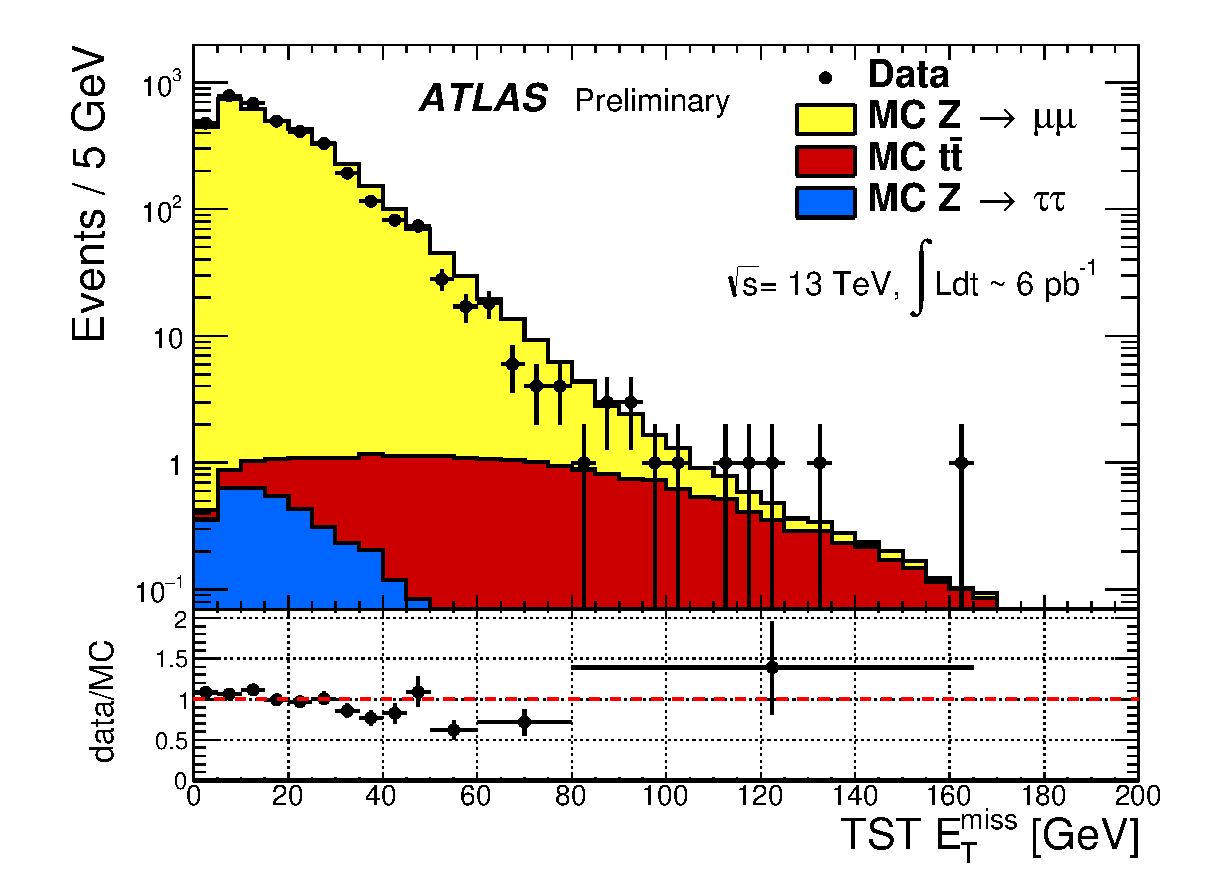
\includegraphics[width=0.45\textwidth]{./figures/object_selection/etmiss_performance_tst_zmm.eps}
    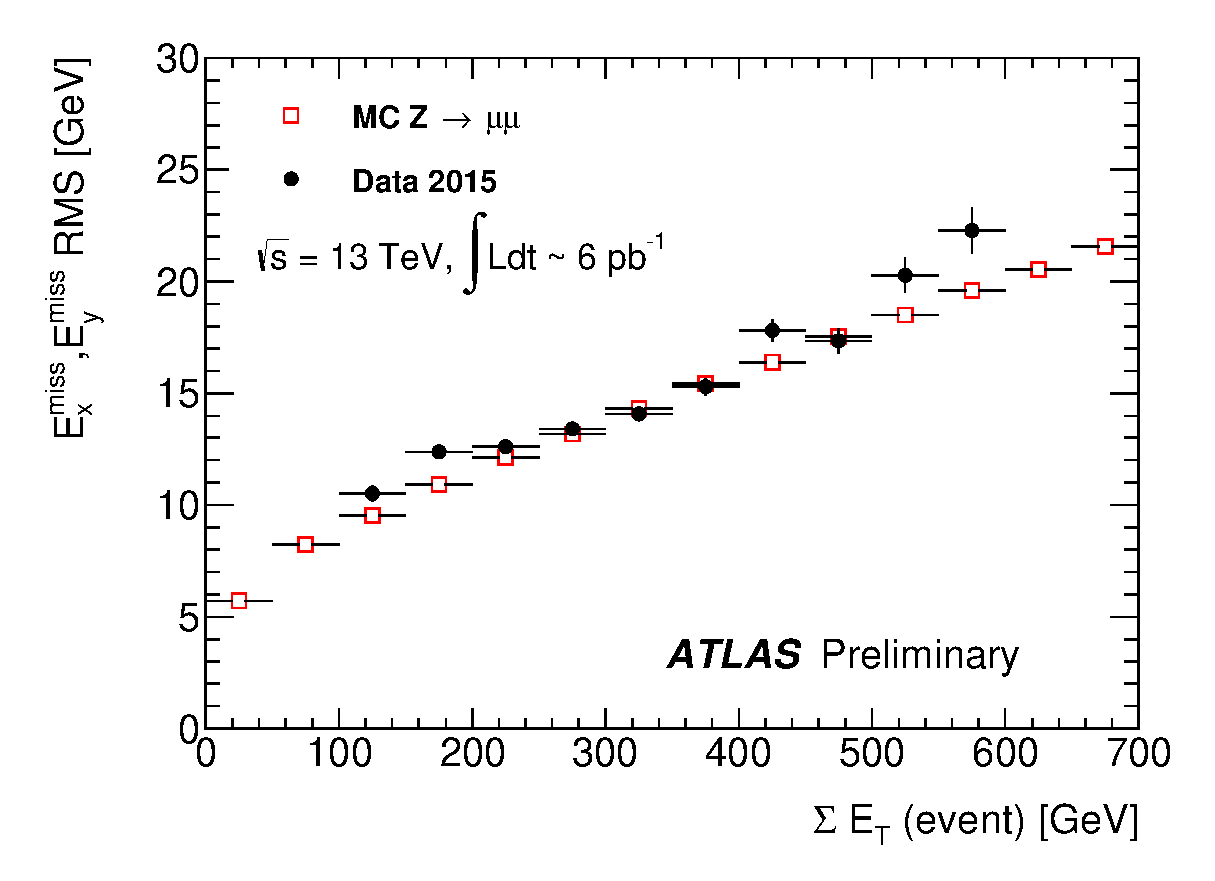
\includegraphics[width=0.45\textwidth]{./figures/object_selection/etmiss_resolution_tst_zmm.eps}
    \caption{Distributions of TST \etmiss{} (left) and the TST $E^\text{miss}_x, E^\text{miss}_y$ resolution (right)
    in $\Z \to \mpmm$ events.~\cite{ATL-PHYS-PUB-2015-027}}\label{fig:object_selection:etmiss}
\end{figure}

\section{Overlap Removal}\label{sec:object_selection:overlap_removal}

It is possible that a detector signature of one particle can pass the reconstruction and identification requirements of multiple objects.
To remove this kind of ambiguity from the analysis an overlap removal is applied.
If two ore more objects are reconstructed within a certain distance \dr{} in the $(\eta - \phi)$ plane, only one object is kept.
First jets are removed, then hadronic $\tau$-leptons, and finally electrons.
Muons are ordered highest and are not removed.
Depending on the object combination, a different \dr{} threshold is used:

\begin{enumerate}
    \item hadronic $\tau$-leptons
        \begin{itemize}
            \item remove jets within $\dr = 0.2$
        \end{itemize}
    \item electrons
        \begin{itemize}
            \item remove jets within $\dr = 0.4$
            \item remove hadronic $\tau$-leptons within $\dr = 0.2$
        \end{itemize}
    \item muons
        \begin{itemize}
            \item remove jets within $\dr = 0.4$
            \item remove hadronic $\tau$-leptons within $\dr = 0.2$
            \item remove electrons within $\dr = 0.2$
        \end{itemize}
\end{enumerate}
\todo{Special electron-jet OLR?}
